\section{Versuchsaufbau}
Die Messung der Lebensdauer der Myonen erfolgt mit einem Szintillationsdetektor, mit dem die Myonen 
nachgewiesen werden können.
Der Detektionsmechanismus beruht dabei auf der Anregung des Szintillatormaterials durch die einfallende ionisierende Strahlung.
Die Anregungsenergie wird in Form von Szintillationslicht wieder abgegeben, welches 
mit zwei Photomultipliern (PMT) detektiert und in ein elektrisches Signal umgewandelt wird.

Es gibt sowohl organische als auch anorganische Szintillatoren, in diesem Versuch wird ein 
organischer Szintillator mit einem Volumen von $\SI{50}{\liter}$ verwendet. Anorganische Szintillatoren sind mit 
Aktivatorzentren dotierte Kristalle, bei denen die Entstehung von Szintillationslicht auf der Bandstruktur des Szintillators 
beruht. Einfallende ionsieriende Strahlung erzeugt freie Elektronen, 
freie Löcher oder Elektron-Loch-Paare, die durch den Festkörper wandern bis sie auf ein 
Aktivatorzentrum treffen. Das Aktivatorzentrum wird angeregt und gibt bei der Rückkehr in den Grundzustand
Licht ab. 
Organische Szintillatoren sind Flüssigkeiten, Kristalle oder polymere Festkörper, in denen Szintillationslicht im UV-Bereich
durch molekulare Übergänge entsteht. Aufgrund der geringen Reichweite von 
UV-Strahlung im Szintillator sind organischen Szintillatoren weitere organische Stoffe als Wellenlängeschieber
beigefügt \cite{szintillatoren1}, \cite{szintillatoren2}. 
Organische Szintillatoren
haben gegenüber anorganischen Szintillatoren den Vorteil, dass sie eine geringere Ansprechzeit haben \cite{szintillatoren3}.

Die verwendete Schaltung ist in Abbildung \ref{fig:schaltung} dargestellt. 
\begin{figure}
    \centering
    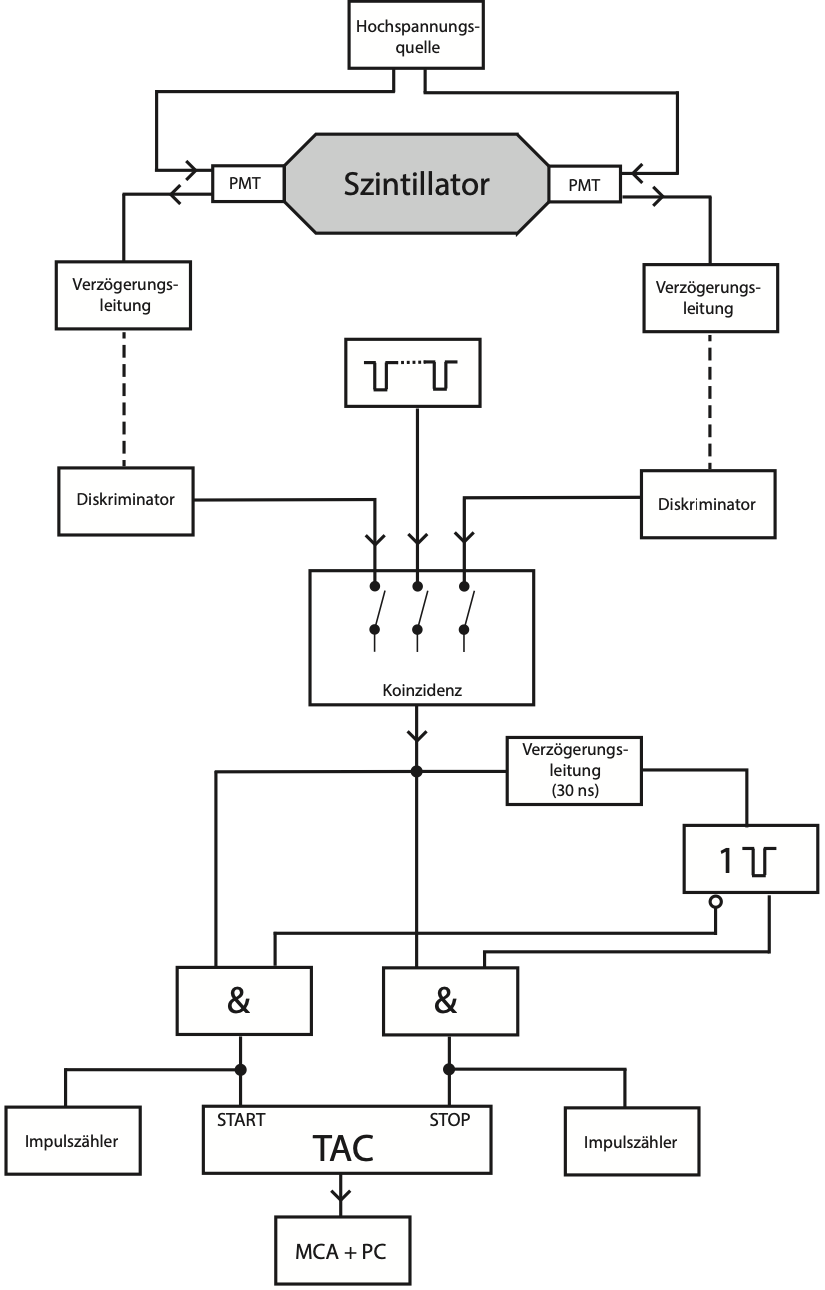
\includegraphics[width=0.6\linewidth]{schaltung.png}
    \caption{Schaltbild des Versuchsaufbaus zur Lebensdauermessung \cite{anleitung}.}
    \label{fig:schaltung}
\end{figure}
Das grundlegende Messprinzip ist, mit einer elektronischen Stoppuhr die Zeit zwischen
dem Eintreffen des Myons im Detektor und dem Zerfall des Myons zu messen. Erwartet werden zwei Signale, 
eins durch das Myon selbst und ein zweites durch die Wechselwirkung der Zerfallsprodukte mit dem 
Szintillatormaterial. 
Die Schwierigkeit bei der Messung der Lebensdauer besteht darin, nur die Ereignisse herauszufiltern, bei 
denen das eintreffende Myon im Szintillator zerfällt.
Problematisch ist dabei, dass die Energie vieler eintreffender Myonen zu groß ist, und sie ohne zu 
zerfallen den Szintillator durchlaufen und somit kein Stoppsignal ausgelöst wird.
Diese Schwierigkeit wird durch die beiden AND-Gatter, die Verzögerungsleitung und den Monoflop überwunden.
Verlässt ein Spannungsimpuls die Koinzidenzschaltung, läuft sie zuerst auf die beiden linken Eingänge
der AND-Gatter. Parallel läuft sie über eine Verzögerungsleitung mit $\Delta t = \SI{30}{\nano\second}$ auf 
den Monoflop. Dieser hat zwei Ausgänge, von denen einer invertiert ist. 
%Nur an dem Ausgang des Monoflops, der mit dem rechten AND-Gatter verbunden ist, liegt Spannung an, wenn 
%am Eingang des Monoflops Spannung anliegt, am anderen Ausgang liegt keine Spannung an. 
%Liegt keine Spannung am Monoflop an, ist die Situation entsprechend umgekehrt. 
Innerhalb der Verzögerungszeit liegt an beiden Eingängen des linken AND-Gatters
Spannung an, wodurch die Zeitmessung mit dem  Time-Amplitude-Converter (TAC)
gestartet wird und der Impulszähler das Signal als Startsignal zählt. Am Monoflop wird eine Suchzeit eingestellt,
innerhalb derer das Stoppsignal eintreffen kann. Trifft innerhalb dieser Suchzeit ein zweites Signal 
auf die Schaltung, liegt durch den invertierten Ausgang des Monoflops am beiden Eingängen des rechten 
AND-Gatters Spannung an, wodurch die Zeitmessung gestoppt wird und ein Stoppimpuls registriert wird. 
Wird innerhalb der Suchzeit kein zweites Signal gemessen, schaltet sich der Monoflop wieder um, sodass 
bei einem erneuten Eintreffen eines Signals wieder an den beiden Eingängen des linken AND-Gatters Spannung
anliegt und ein neues Startsignal aufgenommen werden kann. Über einen Multi-Channel-Analyzer (MCA) wird
die Höhe des vom TAC gemessenen Impulses, der proportioanl zur Zeitdifferenz zwischen Start- und 
Stoppsignal ist, dann Känalen zugewiesen und an den PC weitergegeben, wo ein Histogramm erstellt wird.

Ein weiteres Problem stellt der Untergrund dar, der durch thermisches Rauschen der Photokathoden im Szintillator
ensteht. Die Spannungsimpulse, die bei dieser spontanen Emission von Elektronen entstehen, sind jedoch 
deutlich niedriger als die der eintreffen Myonen. Mit zwei Diskriminatoren werden daher Impulse unterhalb einer 
bestimmten Schwellspannung herausgefiltert und nicht weitergeleitet. Zudem wird eine Koinzidenzschaltung
verwendet. So wird nur ein Signal weitergeleitet, wenn an beiden Seiten dieses Schaltelements 
annähernd gleichzeitig ein Signal eintrifft, was bei spontaner Elektronenemission in den Photokathoden 
statistisch nur äußerst selten der Fall ist.